\documentclass[9pt,hyperref={pdfpagelabels=false},xcolor=table]{beamer}
\usepackage{multicol}

% Contact information: 
%   Jorge M. Cruz-Duarte (jorge.cruz@tec.mx)
%   Nov. 29, 2019

\usepackage{lmodern, ragged2e, CJKutf8, booktabs, subfig,adjustbox, graphicx, amsmath, amssymb, amsthm, amsfonts, mathtools, multirow,wrapfig,lipsum,tikz, tikz-cd,tikz-3dplot,pgfplots,minted}
\usepackage[style=phys]{biblatex}
\usepackage[lined,boxed,vlined,ruled,linesnumbered]{algorithm2e}
\SetKw{Continue}{continue}
\SetKw{Or}{or}
\SetKw{Until}{until}
\addbibresource{bibliography.bib}
\renewcommand{\footnotesize}{\tiny}
\newcommand{\norm}[1]{\left\lVert#1\right\rVert}
\makeatletter
\@newctr{footnote}[page]
\makeatother

\usetheme{CambridgeUS}
\renewcommand{\raggedright}{\leftskip=0pt \rightskip=0pt plus 0cm}

\definecolor{UQPurple}{RGB}{0, 32, 159}
% This is the trademark pruple that UQ uses
\definecolor{UQPurple}{RGB}{81,36,122}
\newcommand{\hl}[1]{{\textcolor{UQPurple}{#1}}}

% Theme setup
\titlegraphic{\includegraphics[scale=0.05]{img/UQ_color_logo.png}}

% \makeatletter
\setbeamertemplate{headline}{%
  \leavevmode%
  \hbox{%
    \begin{beamercolorbox}[wd=\paperwidth,ht=2.5ex,dp=1.125ex]{palette quaternary}%
      \insertsectionnavigationhorizontal{\paperwidth}{}{\hskip0pt plus1filll}
    \end{beamercolorbox}%
  }
}
\setbeamertemplate{footline}{\hspace*{2ex} \insertshortauthor \hfill \textcolor{UQPurple}{\insertshorttitle} \hfill \textbf{\insertframenumber{}} / \inserttotalframenumber \hspace*{2ex}}

\setbeamercolor{item projected}{bg=UQPurple}
\setbeamertemplate{enumerate items}[default]
\setbeamercolor*{enumerate item}{fg=UQPurple}

\setbeamertemplate{navigation symbols}{}
% \setbeamertemplate{footline}[\insertshorttitle frame number]
\setbeamertemplate{bibliography item}[text]
\setbeamertemplate{theorems}[numbered]

\setbeamerfont{title}{series = \bfseries, parent = structure}
\setbeamerfont{frametitle}{series = \bfseries, parent = structure}
\setbeamerfont{headline}{series = \bfseries, size = \tiny, parent = structure}

\setbeamercolor{title}{fg = white, bg = UQPurple}
\setbeamercolor{frametitle}{fg = white, bg = UQPurple}
\setbeamercolor{structure}{fg = UQPurple}
\setbeamercolor{section in head/foot}{fg = black, bg = UQPurple!40}
\setbeamercolor{subsection in head/foot}{fg = black, bg = UQPurple!20}

\setbeamercolor{block title}{use=structure,fg=white,bg=structure.fg!75!black}
\setbeamercolor{block body}{parent=normal text,use=block title,bg=UQPurple!20} %block title.bg!10!bg}
\makeatletter
\def\th@mystyle{%
  \normalfont % body font
  \setbeamercolor{block title example}{bg=orange,fg=white}
  \setbeamercolor{block body example}{bg=orange!20,fg=black}
  \def\inserttheoremblockenv{exampleblock}
}
\makeatother
\theoremstyle{mystyle}
\newtheorem*{remark}{Remark}

\usepackage{tikz,color,xcolor,amsmath,amsfonts,stmaryrd,amssymb,bm}
\usepackage{url}

%Just having a look at what it looks like without it
\setbeamertemplate{background}{\tikz[overlay,remember picture]\node[opacity=0.07]at (current page.center){\includegraphics[width=6cm]{img/UQ_purple_logo.png}};}


\newcommand{\maketitleandtoc}{%
  {%
      \setbeamertemplate{headline}{}%
      \setbeamertemplate{footline}{}%
      \begin{frame}[noframenumbering]%
        \titlepage%
      \end{frame}%
      \begin{frame}[noframenumbering]%
        \frametitle{Outline}%
        \tableofcontents%
      \end{frame}%
    }}

\newcommand{\noheadfoot}[1]{%
  {%
      \setbeamertemplate{headline}{}%
      \setbeamertemplate{footline}{}%
      {#1}
    }
}

\title{Optimizing Gaussian Processes}  
\author[Michael Ciccotosto-Camp]{{\bf Honours Research Project}} 
%\institute{}
\date{
Michael Ciccotosto-Camp - 44302913 \\
}

\begin{document}

\maketitle

\section{Problem Significance}

\begin{frame}
    \frametitle{Problem Setting and Motivation}
    \begin{itemize}
        \item This project focuses on the problem of time series prediction.
        \item Given a data set of $n$ observations $\mathcal{D} = \left\{ \left( x_i , y_i \right) \right\}_{i=1}^{n}$, where each input $x_i \in \mathbb{R}_{>0}$ is a time value and $y_i \in \mathbb{R}$ is a output or experimental observation that acts a function of time, the goal of time series prediction is to try and best predict a value $y_{\star}$ at time $x_{\star}$.
        \item The idea of studying time series prediction came from a research group from the Gatton campus, lead by Andries Potgieter, analysing crop growth from previous seasons to forecast when certain phenological stages will take place in the current harvest.
    \end{itemize}
    \begin{figure}
        \centering
        \includegraphics[scale=0.18]{img/yan_wheat_GPR_plot.png}
    \end{figure}
\end{frame}

\section{Gaussian Processes}

\begin{frame}
    \frametitle{Introduction to Gaussian Processes}
    \begin{itemize}
        \item Originally, Potgieter's team surveyed a number of different parameteric models to carry out forecasting. However, the parameteric models we serverely limited in their ability to inform when key phenological stages would take place. After seeing the success of applying GPs to other remote senesing tasks investigated the use of GPs in their own research to find that they could produce much higher resolution predictions from which they could infer a far richer phenological timeline.
        \item A Gaussian Process (GP) is a collection of random variables with index set $I$, such that every finite subset of random variables has a joint Gaussian distribution.
        \item A GP is completely characterized by a mean function $m : X \to \mathbb{R}$ and a kernel $k : X \times X \to \mathbb{R}$.
    \end{itemize}
    \begin{align*}
        m(\bm{x})           & = \mathbb{E} \left[ f(\bm{x}) \right]                                          \\
        k (\bm{x}, \bm{x'}) & = \mathbb{E} \left[ (f(\bm{x}) - m(\bm{x})) (f(\bm{x'}) - m(\bm{x'})) \right].
    \end{align*}
    \begin{itemize}
        \item In this context, think of the kernel as a function that provides some notion of similarity between points.
    \end{itemize}
\end{frame}

\begin{frame}
    \frametitle{Predictions}
    \begin{itemize}
        \item The aim of GPs is to find a suitable mean function, $m$, for which we can then predict inputs from outside the observed values, $\bm{X_{\star}}$. This requires an understand of the function $f$.
        \item Adopting the notation $\left( \bm{K}_{\bm{W} \bm{W}'} \right)_{i,j} \triangleq k \left( \bm{w}_i , \bm{w}_j' \right)$, when attempting to model our value function we usually do not have access to the value function itself but a noisy version thereof, $y = f(\bm{x}) + \varepsilon$ where $\varepsilon \sim \mathbb{N} (0, \sigma_n^2)$ meaning the prior on the noisy values becomes $\operatorname{cov} (\bm{y}) = \bm{K_{XX}} + \sigma_n^2 \bm{I}$.
        \item Using the assumption that our data can be modelled as a Gaussian process, we can write out the new distribution of the observed noisy values along the points at which we wish to test the underlying function as
              \[
                  \begin{bmatrix}
                      \bm{y} \\
                      \bm{f}_{\star}
                  \end{bmatrix}
                  \sim \mathbb{N}
                  \begin{pmatrix}
                      \bm{0}, &
                      {
                              \begin{bmatrix}
                                  \bm{K_{XX}} + \sigma_n^2 \mathbb{I}_{n \times n} & \bm{K_{X_{\star}X}^{\intercal}} \\
                                  \bm{K_{X_{\star}X}}                              & \bm{K_{X_{\star}X_{\star}}}
                              \end{bmatrix}
                          }
                  \end{pmatrix}.
              \]
        \item The mean and covariance can then be computed as
              \begin{align*}
                  \overline{\bm{f}_{\star}}           & \triangleq \bm{K_{X_{\star}X}} \left[ \bm{K_{XX}} + \sigma_n^2 \mathbb{I}_{n \times n} \right]^{-1} \bm{y}                                                \\
                  \operatorname{cov} (\bm{f}_{\star}) & = \bm{K_{X_{\star}X_{\star}}} - \bm{K_{X_{\star}X}} \left[ \bm{K_{XX}} + \sigma_n^2 \mathbb{I}_{n \times n} \right]^{-1} \bm{K_{X_{\star}X}}^{\intercal}.
              \end{align*}
    \end{itemize}
\end{frame}

\begin{frame}
    \frametitle{Unoptimized GPR}
    {\centering
        \begin{minipage}{.9\linewidth}
            \begin{algorithm}[H]
                \caption{Unoptimized GPR}
                \SetAlgoLined
                \DontPrintSemicolon
                \SetKwInOut{Input}{input}\SetKwInOut{Output}{output}

                \Input{Observations $\bm{X}, \bm{y}$ and a test input $\bm{x}_{\star}$.}
                \Output{A prediction $\overline{f_{\star}} $ with its corresponding variance $ \mathbb{V} \left[ f_{\star} \right]$.}
                \BlankLine
                $\bm{L} = \operatorname{cholesky} \left( \bm{K_{XX}} + \sigma_n^2 \mathbb{I}_{n \times n} \right)$\;
                $\bm{\alpha} = \operatorname{lin-solve} \left( \bm{L}^{\intercal} , \operatorname{lin-solve} \left( \bm{L}, \bm{y} \right) \right)$\;
                $\overline{f_{\star}} = \bm{K_{x_{\star} X}} \bm{\alpha}$\;
                $\bm{v} = \operatorname{lin-solve} \left( \bm{L}, \bm{K_{x_{\star} X}} \right)$\;
                $\mathbb{V} \left[ f_{\star} \right] = \bm{K_{x_{\star} x_{\star}}} - \bm{v}^{\intercal} \bm{v}$\;
                \Return{$\overline{f_{\star}} , \mathbb{V} \left[ f_{\star} \right]$}
                \BlankLine
            \end{algorithm}
        \end{minipage}
        \par
    }
\end{frame}

\begin{frame}
    \frametitle{Problems with Unoptimized GPR}
    {\centering
        \begin{minipage}{.9\linewidth}
            \begin{algorithm}[H]
                \caption{Unoptimized GPR}
                \SetAlgoLined
                \DontPrintSemicolon
                \SetKwInOut{Input}{input}\SetKwInOut{Output}{output}

                \Input{Observations $\bm{X}, \bm{y}$ and a test input $\bm{x}_{\star}$.}
                \Output{A prediction $\overline{f_{\star}} $ with its corresponding variance $ \mathbb{V} \left[ f_{\star} \right]$.}
                \BlankLine
                \textcolor{red}{$\bm{L} = \operatorname{cholesky} \left( \bm{K_{XX}} + \sigma_n^2 \mathbb{I}_{n \times n} \right)$}\;
                $\bm{\alpha} = \operatorname{lin-solve} \left( \bm{L}^{\intercal} , \operatorname{lin-solve} \left( \bm{L}, \bm{y} \right) \right)$\;
                $\overline{f_{\star}} = \bm{K_{x_{\star} X}} \bm{\alpha}$\;
                $\bm{v} = \operatorname{lin-solve} \left( \bm{L}, \bm{K_{x_{\star} X}} \right)$\;
                $\mathbb{V} \left[ f_{\star} \right] = \bm{K_{x_{\star} x_{\star}}} - \bm{v}^{\intercal} \bm{v}$\;
                \Return{$\overline{f_{\star}} , \mathbb{V} \left[ f_{\star} \right]$}
                \BlankLine
            \end{algorithm}
        \end{minipage}
        \par
    }
    \begin{itemize}
        \item \textcolor{red}{Line 1} can be incredibly slow as computing $\bm{K_{XX}}$ and performing a Cholesky decomposition scale poorly as the number of inputs, $n$, grows.
    \end{itemize}
\end{frame}

\section{Nystrom}

\begin{frame}
    \frametitle{Nystrom Approximation}
    \begin{itemize}
        \item One technique to speed up the computation of $\bm{K_{XX}}$ is to use a Nystrom approximation.
        \item The Nystrom method we seek a matrix $\bm{Q}\in \mathbb{R}^{n \times k}$ that satisfies $\norm{\bm{A} - \bm{Q} \bm{Q}^{\ast} \bm{A}}_{F} \leq \varepsilon$, where $\bm{A} \in \mathbb{R}^{n \times n}$ is positive semi definite matrix, to form the rank$-k$ approximation
              \begin{align*}
                  \bm{A} & \simeq \bm{Q} \bm{Q}^{\ast} \bm{A}                                                                                                                                \\
                         & \simeq \bm{Q} \left( \bm{Q}^{\ast} \bm{A} \bm{Q} \right) \bm{Q}^{\ast}                                                                                            \\
                         & = \bm{Q} \left( \bm{Q}^{\ast} \bm{A} \bm{Q} \right) \left( \bm{Q}^{\ast} \bm{A} \bm{Q} \right)^{\dagger} \left( \bm{Q}^{\ast} \bm{A} \bm{Q} \right) \bm{Q}^{\ast} \\
                         & \simeq \left( \bm{A} \bm{Q} \right) \left( \bm{Q}^{\ast} \bm{A} \bm{Q} \right)^{\dagger} \left( \bm{Q}^{\ast} \bm{A} \right).
              \end{align*}
        \item A matrix $\bm{Q}$ that satisfies the above conditions can be built using through a very popular column sampling technique.
        \item As the name suggests, the matrix $\bm{Q}$ essentially samples and rescales columns from $\bm{A}$ using a probability distribution $\left\{ p_i \right\}_{i=1}^{n}$.
        \item When $\bm{Q}$ is constructed in this manner, it is usually referred to as a sketching matrix and denoted $\bm{S}$.
    \end{itemize}
\end{frame}

\section{Random Fourier Features}

\begin{frame}
    \frametitle{Random Fourier Feature Approximation}
    \begin{itemize}
        \item The other technique investigated to speed up the computation of $\bm{K_{XX}}$ is the Random Fourier Feature (RFF) approximation.
        \item The main idea is instead of using a kernel function to implicitly lift data into a higher dimensional feature space, an explicit feature map $\varphi : \mathbb{R}^d \to \mathbb{R}^D$ could be used to approximate $k$ as $k \left( \bm{x} , \bm{y} \right) = \langle \Phi (\bm{x}) , \Phi (\bm{y}) \rangle_{\mathbb{R}^N} \simeq \langle \varphi (\bm{x}) , \varphi (\bm{y}) \rangle_{\mathbb{R}^D}$ where $D$ is chosen so that $n \gg  D$. Once $\varphi (\bm{x}_i)$ has been computed for each $\bm{x}_i$, every entry of the Gram matrix can be swiftly approximated as $\bm{K}_{ij} = \bm{K}_{ji} \simeq \langle \varphi (\bm{x}_i) , \varphi (\bm{y}_j) \rangle_{\mathbb{R}^D}$.
        \item The RFF technique hinges on Bochners theorem which characterises positive definite functions (namely kernels) and states that any positive definite functions can be represented as
              \[
                  k \left( \bm{x} - \bm{y} \right) = k \left( \bm{x} - \bm{y} \right) = \int_{\mathbb{C}^d} \exp \left( i \langle \bm{\omega} , \bm{x} - \bm{y} \rangle \right) \mu_k \left( d \bm{\omega} \right)
              \]
              where $\mu_k$ is a positive finite measure on the frequencies of $\bm{\omega}$.
    \end{itemize}
\end{frame}

\begin{frame}
    \begin{figure}
        \centering
        \frametitle{Infrared Spectroscopy and Mass Spectrum Data}
        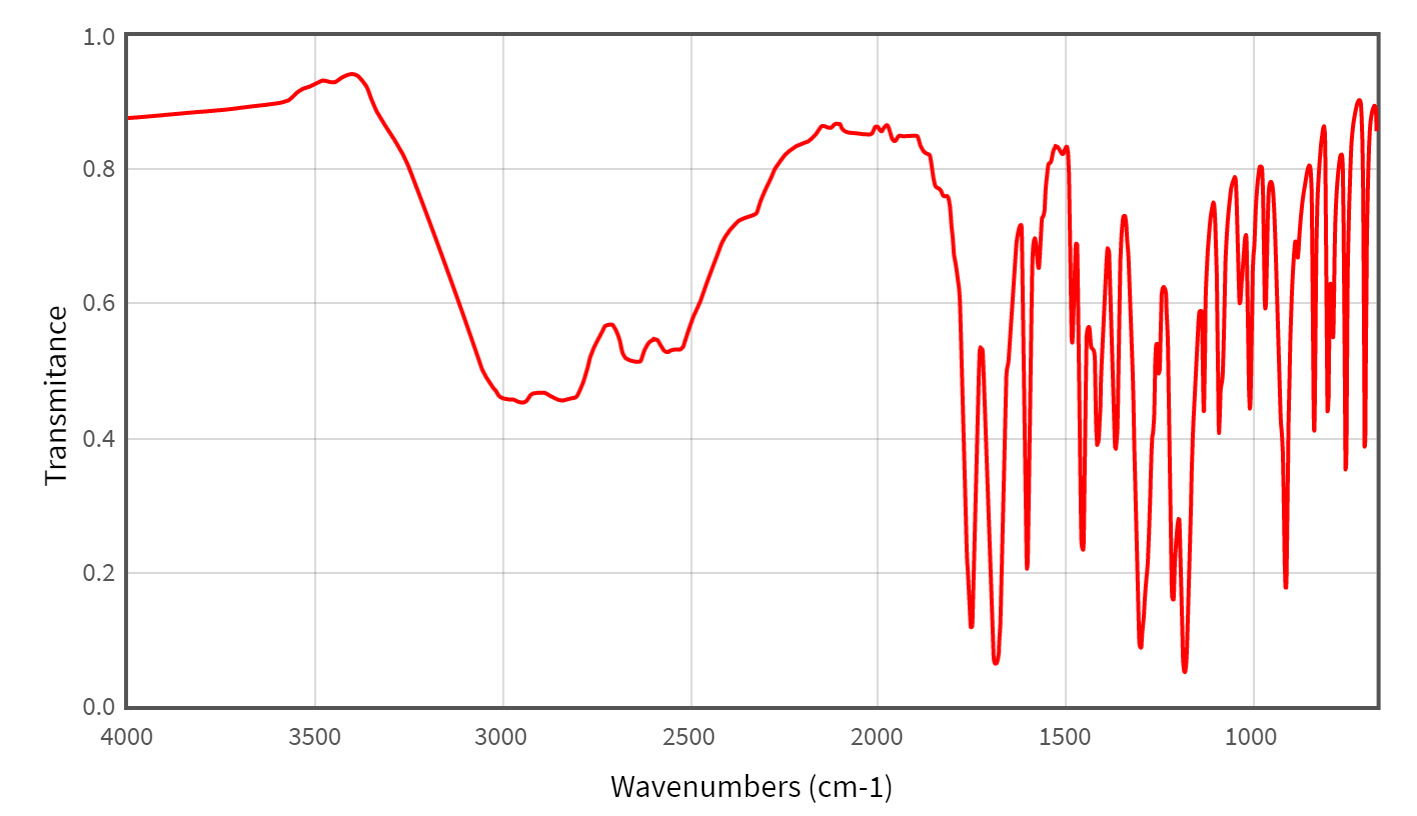
\includegraphics[scale=0.35]{aspirin_IR}
        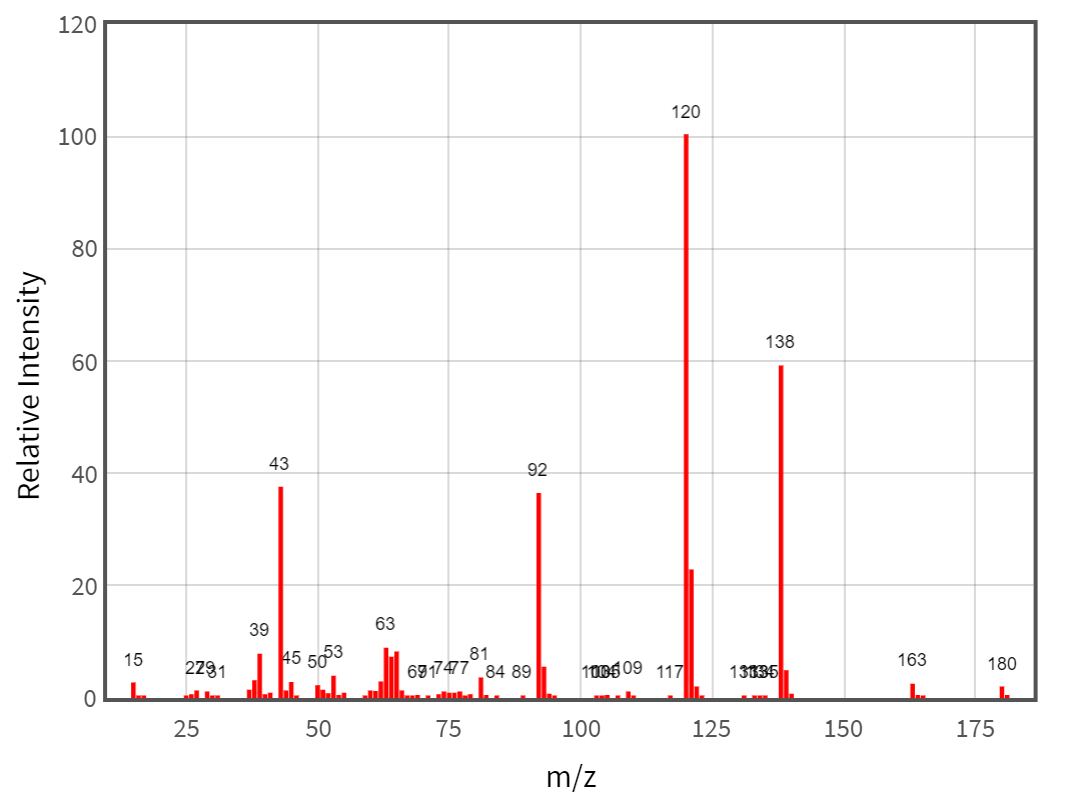
\includegraphics[scale=0.35]{MS _data_aspirin}
    \end{figure}
    \begin{itemize}
        \item \textbf{Project Goal:} Develop a deep learning model to accurately predict functional groups based off Infrared (IR) and Mass Spectrometry (MS) data \footfullcite{NIST}. Main focus will be on Multi-layer Perceptrons (MLPs).
    \end{itemize}
\end{frame}

\end{document}

